\section{Introducción a las Comunicaciones}

\subsection{Motivación y Conceptos Fundamentales}

En términos primitivos, la comunicación consiste en la transferencia de información entre distintos puntos mediante la variación de una propiedad física (voltaje, corriente, señales electromagnéticas) a través de un medio de transmisión. Con el avance de la tecnología y la democratización de los sistemas digitales, las comunicaciones han evolucionado rápidamente, impulsadas por los gobiernos en contextos de defensa y seguridad, y por la industria en contextos de comercio y entretenimiento. La convergencia de estas motivaciones ha dado lugar a un ecosistema altamente desarrollado.

\begin{definicion}[Red de Computadoras]
Una red de computadoras es un conjunto de computadoras autónomas interconectadas mediante una sola tecnología. Se considera que dos computadoras están interconectadas si tienen la capacidad de intercambiar información. La interconexión física puede realizarse a través de medios guiados (cobre, fibra óptica) o no guiados (enlaces de radio, microondas, satélites).
\end{definicion}

Es indispensable establecer la frontera conceptual entre una red de computadoras y un sistema distribuido.

\begin{obs}[Red de Computadoras vs. Sistema Distribuido]
En un \textbf{sistema distribuido}, un conjunto de computadoras independientes se presenta ante sus usuarios como un único sistema coherente, empleando una capa de software (middleware) que provee cohesión y transparencia. En una \textbf{red de computadoras}, esta coherencia no existe por diseño: las máquinas exponen sus particularidades (hardware y sistema operativo) y los usuarios o aplicaciones deben gestionar explícitamente la comunicación con los equipos remotos. La diferencia fundamental recae en la abstracción provista por el software, no en el hardware subyacente.
\end{obs}

\subsection{Hardware de Red}

Al hablar de hardware de red nos referimos a las cuestiones técnicas implicadas en el diseño e implementación de dichas redes en términos de componentes físicos y su interacción. Existen muchos tipos de redes y muchas variaciones de cada tipo, por lo que encontrar categorías en las cuales caigan absolutamente todas las redes es casi imposible. De este modo nos concentraremos en solamente dos aspectos: la tecnología de transmisión y la escala.

\subsubsection{Tecnología de Transmisión}

Hablando en sentido general, existen dos tipos de tecnología de transmisión que se emplean de forma predominante en la actualidad: los enlaces de difusión (broadcast) y los enlaces de punto a punto.

\begin{itemize}
  \item \textbf{Enlaces de difusión (Broadcast):} 
  En este tipo de redes, todas las máquinas comparten un único canal de comunicación. Los paquetes enviados por una máquina son recibidos por todas las demás máquinas de la red. Cada paquete contiene un campo de dirección que especifica el destinatario. Cuando una máquina recibe un paquete, verifica esta dirección; si el paquete está destinado a ella, lo procesa, de lo contrario, lo ignora. Los sistemas de difusión soportan la transmisión a todos los destinos simultáneamente utilizando un código de dirección especial (operación de broadcast) y, frecuentemente, la transmisión a un subconjunto de máquinas (operación de multicast). Un ejemplo típico de enlace de difusión son las redes inalámbricas.

  \item \textbf{Enlaces de punto a punto:} 
  Conectan pares individuales de máquinas. Para transmitir un paquete desde el origen hasta el destino en una red de punto a punto, el mensaje puede tener que visitar una o más máquinas intermedias. Dado que frecuentemente existen múltiples rutas de diferentes longitudes, los algoritmos de enrutamiento resultan fundamentales en la arquitectura de estas redes. La transmisión de punto a punto con un solo emisor y un solo receptor se denomina unidifusión (unicast).
\end{itemize}

\subsubsection{Escala de la Red}

El segundo criterio fundamental para la clasificación de redes es su escala física, es decir, la distancia que abarca la comunicación. La escala determina las tecnologías de hardware, los medios de transmisión y los protocolos de acceso al medio requeridos. Los sistemas interconectados se clasifican según su distancia en las siguientes categorías principales:

\begin{itemize}
  \item \textbf{Redes de Área Personal (PAN, Personal Area Network):} 
  Permiten la comunicación de dispositivos dentro del rango de acción de una persona, típicamente del orden de 1 metro. El caso de uso habitual es la interconexión de periféricos de computadora o dispositivos portátiles de forma inalámbrica.

  \item \textbf{Redes de Área Local (LAN, Local Area Network):} 
  Redes que operan dentro de un único edificio o campus, abarcando distancias de decenas de metros hasta un kilómetro. Debido a su extensión limitada, el tiempo de transmisión en el peor de los casos es acotado y conocido, lo que permite latencias bajas, bajas tasas de error y altos anchos de banda. Se dividen principalmente en:
  \begin{itemize}
    \item \textbf{Alámbricas:} Dominadas por la tecnología Ethernet (IEEE 802.3), operando generalmente bajo una topología conmutada mediante el uso de switches que vinculan enlaces de punto a punto.
    \item \textbf{Inalámbricas:} Dominadas por el estándar WiFi (IEEE 802.11), donde las máquinas se comunican mediante un medio de difusión hacia un punto de acceso (AP, Access Point).
  \end{itemize}

  \item \textbf{Redes de Área Metropolitana (MAN, Metropolitan Area Network):} 
  Abarcan el área geográfica de una ciudad, del orden de 10 kilómetros. El ejemplo clásico es la red de televisión por cable, la cual fue readaptada para proveer conectividad a Internet de dos vías distribuyendo el espectro.

  \item \textbf{Redes de Área Amplia (WAN, Wide Area Network):} 
  Cubren extensiones geográficas masivas, como un país o continente, en un rango de 100 a 1000 kilómetros. Su diseño introduce una separación arquitectónica estricta entre dos componentes:
  \begin{itemize}
    \item Los \textbf{hosts}: Computadoras dedicadas a ejecutar los programas de aplicación.
    \item La \textbf{subred de comunicación}: Encargada exclusivamente del transporte de mensajes entre hosts. A su vez, está conformada por líneas de transmisión (que mueven los bits, ya sea mediante cobre, fibra o enlaces de radio) y elementos de conmutación (enrutadores o routers, que deciden la línea de salida para cada paquete entrante).
  \end{itemize}
  A diferencia de las LAN, la subred y los hosts de una WAN generalmente pertenecen a entidades distintas, por ejemplo, una empresa administra los hosts y un proveedor de servicios de red (ISP, Internet Service Provider) opera la subred.

  \item \textbf{Interredes (Internetworks):} 
  Una interred se forma cuando se interconectan múltiples redes individuales que pueden utilizar tecnologías subyacentes incompatibles. La interconexión se logra a través de puertas de enlace (gateways). Los routers operan en la capa de red como puertas de enlace para traducir y encaminar los paquetes entre las distintas redes. La Internet global constituye el ejemplo primario de una interred.
\end{itemize}

\begin{obs}[VPNs]
Una red privada virtual (VPN, Virtual Private Network) es un tipo de interred que permite a los usuarios conectarse a una red privada a través de una red pública, como Internet. Esto se logra mediante la creación de un ``túnel'' cifrado que protege la información transmitida. Las VPNs son ampliamente utilizadas para garantizar la seguridad y privacidad de los datos, especialmente en entornos corporativos y para el acceso remoto a redes privadas. En otras palabras, una VPN simula una red privada sobre una infraestructura pública, permitiendo a los usuarios acceder a recursos de la red privada como si estuvieran físicamente presentes en ella.
\end{obs}

\subsection{Software de Red}

Para reducir la complejidad de su diseño, la mayoría de las redes modernas están organizadas de forma altamente estructurada mediante una jerarquía de capas o niveles. Cada capa se construye a partir de la que está debajo de ella. El propósito de cada capa es ofrecer ciertos servicios a las capas superiores, ocultando los detalles relacionados con la implementación de dichos servicios.

\subsubsection{Jerarquías de Protocolos}

La comunicación en red se fundamenta en un modelo de capas en el cual las entidades que conforman la misma capa en diferentes máquinas se denominan pares (peers). Los pares pueden ser procesos de software, dispositivos de hardware o incluso seres humanos. La comunicación no ocurre de forma directa y horizontal entre las capas superiores, sino que los datos y la información de control descienden a través de las capas hasta alcanzar el medio físico.

Entre cada par de capas adyacentes existe una \textbf{interfaz}, la cual define las operaciones y servicios primitivos que la capa inferior pone a disposición de la capa superior. Una interfaz limpia y bien definida permite reemplazar la implementación de una capa sin afectar al resto del sistema, abstrayendo los detalles de la implementación en la capa inferior.

\begin{definicion}[Protocolo]
Un protocolo es un conjunto de reglas y convenciones que rigen el formato, el significado y la sincronización de los paquetes o mensajes intercambiados entre entidades pares para establecer la comunicación dentro de una misma capa.
\end{definicion}

\begin{definicion}[Arquitectura de Red y Pila de Protocolos]
Una arquitectura de red es el conjunto de capas y protocolos subyacentes que definen el funcionamiento de la red. Ni los detalles de implementación ni la especificación interna de las interfaces forman parte de la arquitectura. La lista de los protocolos específicos utilizados por un sistema, con un protocolo por capa, se denomina pila de protocolos.
\end{definicion}

\subsubsection{Aspectos de Diseño para las Capas}

Algunos de los aspectos clave de diseño que ocurren en las redes de computadoras están presentes en las diversas capas. A continuación mencionaremos brevemente los más importantes.

\begin{itemize}
  \item \textbf{Confiabilidad:} La confiabilidad de un servicio se refiere a la capacidad de garantizar la entrega de los datos sin pérdidas, errores o duplicaciones. Esto se logra mediante mecanismos como acuses de recibo (ACKs), retransmisiones, control de flujo, redundancia, etc... Es fundamental sabiendo que las comunicaciones pueden estar sujetas a interferencias, fallos de hardware o congestión en la red (medios imperfectos). Otro aspecto de la confiabilidad consiste en encontrar una ruta funcional a través de la red, lo cual puede implicar el uso de algoritmos de \textbf{enrutamiento}.
  \item \textbf{Direccionamiento y nombramiento:} Dado que existen múltiples computadoras interconectadas, cada capa necesita un mecanismo para identificar unívocamente a los emisores y receptores involucrados en una transmisión específica. Este proceso se conoce como direccionamiento en las capas inferiores y nombramiento en las capas superiores.
  \item \textbf{Control de flujo y asignación de recursos:} Es imperativo contar con mecanismos que eviten que un emisor rápido sature o inunde de datos a un receptor lento, resolviéndose usualmente mediante retroalimentación. Asimismo, la red debe asignar los recursos compartidos (como el ancho de banda) de manera eficiente y gestionar la \textbf{congestión} cuando la cantidad de información a transmitir supera la capacidad del sistema.
  \item \textbf{Escalabilidad y adaptabilidad:} Con esto nos referimos a la capacidad de la red para crecer y adaptarse a un número creciente de usuarios, dispositivos y tráfico sin degradar significativamente el rendimiento, al igual que la posibilidad de mutar y adoptar nuevas tecnologías. Esto implica diseñar protocolos y arquitecturas que puedan manejar eficientemente el aumento de la carga, la expansión geográfica y la evolución de la red.
  \item \textbf{Seguridad:} La seguridad en las comunicaciones de red abarca la protección de los datos y la infraestructura contra accesos no autorizados. Esto incluye la implementación de cifrado, autenticación, control de acceso, detección de intrusiones y políticas de seguridad para garantizar la confidencialidad e integridad de la información transmitida. 
\end{itemize}

Existen otros aspectos de diseño que son importantes en ciertas capas que no hemos mencionado, más no significa que sean menos importantes. Por ejemplo, la eficiencia espectral (maximizar la cantidad de datos transmitidos por unidad de tiempo) es un aspecto crítico en las capas físicas y de enlace de datos, mientras que la latencia y el ancho de banda son consideraciones clave en las capas superiores.

\subsubsection{Tipos de Servicios}

Una capa puede ofrecer a la capa superior dos tipos fundamentales de servicio:

\begin{itemize}
  \item \textbf{Servicio orientado a la conexión:} Modelado a partir del sistema telefónico. El usuario del servicio primero establece una conexión, la utiliza y finalmente la libera. Se comporta como un canal dedicado que generalmente preserva el orden de los datos. Se divide en dos variantes:
  \begin{itemize}
    \item \textbf{Secuencias de mensajes:} Conserva los límites físicos de los mensajes (por ejemplo, dos mensajes de 1024 bytes se reciben como dos unidades distintas).
    \item \textbf{Flujo de bytes:} La conexión es un flujo continuo sin límites en los mensajes (por ejemplo, 2048 bytes recibidos no revelan si fueron enviados juntos o en fragmentos).
  \end{itemize}

  \item \textbf{Servicio sin conexión:} Modelado a partir del sistema postal. Cada mensaje lleva la dirección de destino completa y es enrutado a través de nodos intermedios de forma independiente a los mensajes subsecuentes. Cuando no incluye confirmación de recepción, este modelo se denomina \textbf{servicio de datagramas}.
\end{itemize}

Cada uno de estos servicios puede caracterizarse según su \textbf{confiabilidad}. Un servicio es confiable si garantiza la entrega de los datos sin pérdidas, habitualmente mediante el uso de acuses de recibo (ACKs). La confirmación de recepción introduce sobrecarga y retardo temporal en la red. Aplicaciones como la transferencia de archivos exigen flujos de bytes confiables, mientras que aplicaciones multimedia en tiempo real, como la voz sobre IP (VoIP), toleran la pérdida esporádica de datos pero exigen la mínima latencia que proveen los servicios no confiables (sin confirmación).

\subsubsection{Primitivas de Servicios}

Un servicio se especifica formalmente mediante un conjunto de primitivas disponibles a los procesos de usuario. Estas primitivas indican al servicio que ejecute alguna acción o que informe sobre la acción de una entidad par. En un servicio simple orientado a la conexión. Las primitivas típicas son: \texttt{connect, send, receive, listen, accept, disconnect}. En un servicio sin conexión, las primitivas típicas son: \texttt{send, receive}.

\begin{obs}[Servicios vs. Protocolos]
Un \textbf{servicio} es un conjunto de primitivas que una capa proporciona a la capa que está sobre ella. Define la semántica de la interfaz y estipula qué operaciones están disponibles, pero no cómo se implementan. Por el contrario, un \textbf{protocolo} es un conjunto de reglas que rigen el formato y el significado de los paquetes intercambiados entre entidades pares. Las entidades utilizan los protocolos para implementar las definiciones de los servicios ofrecidos. El servicio y el protocolo son ortogonales, un protocolo puede ser modificado o reemplazado sin alterar el servicio visible para la capa superior.
\end{obs}

\subsection{Modelos de Referencia}

La arquitectura de las redes de computadoras se organiza y estandariza mediante modelos de referencia. Los dos modelos que analizaremos son el modelo OSI y el modelo TCP/IP. Aunque ya casi no se utilizan los protocolos asociados con el modelo OSI, el modelo en sí es bastante general y sigue siendo válido. Asimismo, las características en cada nivel siguen siendo muy importantes. El modelo TCP/IP tiene las propiedades opuestas: el modelo en sí no se utiliza mucho, pero los protocolos son usados ampliamente. Por esta razón veremos ambos elementos con detalle. Además, algunas veces podemos aprender más de los fracasos que de los éxitos.

\subsubsection{El Modelo de Referencia OSI}

El modelo OSI (Open Systems Interconnection), propuesto por la Organización Internacional de Normalización (ISO), consta de siete capas. Su diseño se basa en 5 principios fundamentales:

\begin{enumerate}
  \item Se debe crear una capa en donde se requiera un nivel diferente de abstracción.
  \item Cada capa debe realizar una función bien definida.
  \item La función de cada capa se debe elegir teniendo en cuenta la definición de protocolos estandarizados internacionalmente.
  \item Es necesario elegir los límites de las capas de modo que se minimice el flujo de información a través de las interfaces.
  \item La cantidad de capas debe ser suficiente como para no tener que agrupar funciones distintas en la misma capa. Además, debe ser lo bastante pequeña como para que la arquitectura no se vuelva inmanejable.
\end{enumerate}

Las siete capas del modelo OSI son:

\begin{enumerate}
  \item \textbf{Capa Física:} Encargada de la transmisión de bits puros a través de un canal de comunicación. Define las especificaciones eléctricas, mecánicas y de temporización del medio de transmisión.
  \item \textbf{Capa de Enlace de Datos:} Transforma un medio de transmisión puro en una línea libre de errores para la capa de red. Divide los datos en tramas, administra el acceso al medio y gestiona el control de errores y de flujo. Otra cuestión que surge en la capa de enlace de datos (y en la mayoría de las capas superiores) es cómo evitar que un transmisor rápido inunde de datos a un receptor lento. Tal vez sea necesario algún mecanismo de regulación de tráfico para notificar al transmisor cuando el receptor puede aceptar más datos.
  \item \textbf{Capa de Red:} Controla el funcionamiento de la subred. Su función principal es el enrutamiento de paquetes desde el origen hasta el destino, gestionando la congestión y permitiendo la interconexión de redes heterogéneas. En las redes de difusión, el problema de encaminamiento es simple, por lo que con frecuencia la capa de red es delgada o incluso inexistente.
  \item \textbf{Capa de Transporte:} Acepta los datos de la capa de sesión, los divide en unidades más pequeñas si es necesario y asegura que todos los fragmentos lleguen correctamente al otro extremo. Es la primera capa verdaderamente de extremo a extremo (end-to-end).
  \item \textbf{Capa de Sesión:} La capa de sesión permite a los usuarios en distintas máquinas establecer sesiones entre ellos. Las sesiones ofrecen varios servicios, incluyendo el control del diálogo (llevar el control de quién va a transmitir), el manejo de tokens (evitar que dos partes intenten la misma operación crítica al mismo tiempo) y la sincronización (usar puntos de referencia en las transmisiones extensas para reanudar desde el último punto de referencia en caso de una interrupción).
  \item \textbf{Capa de Presentación:} Se enfoca en la sintaxis y la semántica de la información transmitida, gestionando la representación y codificación abstracta de los datos.
  \item \textbf{Capa de Aplicación:} Contiene los protocolos de alto nivel que los usuarios y las aplicaciones necesitan para la comunicación en red (ej. HTTP, FTP, SMTP).
\end{enumerate}

La siguiente figura ilustra el modelo OSI y sus capas.

\begin{figure}[h]
  \centering
  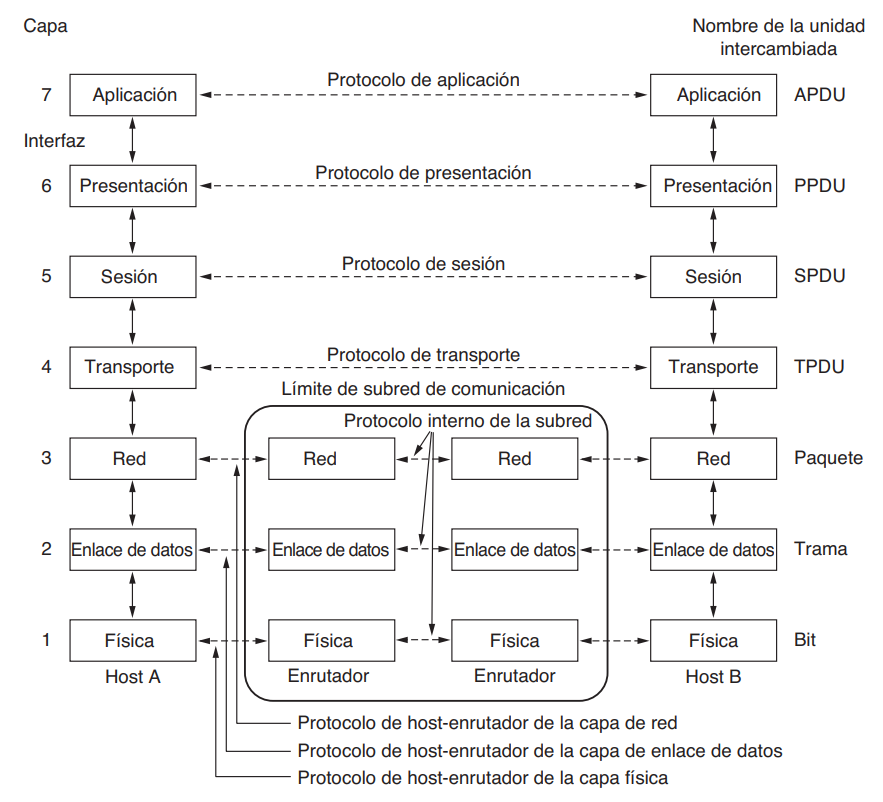
\includegraphics[width=0.90\textwidth]{imgs/1.2.png}
\end{figure}

\subsubsection{El Modelo de Referencia TCP/IP}

El modelo TCP/IP, desarrollado inicialmente por ARPA (Advanced Research Projects Agency) para la red ARPANET, se diseñó con el objetivo principal de conectar múltiples redes de manera transparente y garantizar la supervivencia de la comunicación frente a fallos en el hardware de la subred. El mismo se definió por primera vez en 1974 por Cerf y Kahn. 

Consta de cuatro capas:

\begin{enumerate}
  \item \textbf{Capa de Enlace (Host-to-Network):} Es la capa más baja. En el modelo original no está estrictamente definida como una capa funcional, sino como una interfaz que indica que el host debe conectarse a la red utilizando algún protocolo que le permita enviar paquetes IP.
  \item \textbf{Capa de Interred (Internet):} Eje central de la arquitectura. Su función es inyectar paquetes en cualquier red y que viajen de manera independiente hacia el destino. Incluso pueden llegar en un orden totalmente diferente al orden en que se enviaron, en cuyo caso es responsabilidad de las capas más altas volver a ordenarlos, si se desea una entrega en orden. La capa de interred define un formato de paquete y un protocolo oficial llamado IP (Internet Protocol), además de un protocolo complementario llamado ICMP (Internet Control Message Protocol) que le ayuda a funcionar. La tarea de la capa de interred es entregar los paquetes IP a donde se supone que deben ir. Aquí el ruteo de los paquetes es sin duda el principal aspecto, al igual que la congestión (aunque el IP no ha demostrado ser efectivo para evitar la congestión).
  \item \textbf{Capa de Transporte:} Diseñada para permitir que las entidades pares en los nodos de origen y destino mantengan una conversación de extremo a extremo. Define dos protocolos principales: 
  \begin{itemize}
    \item TCP (Transmission Control Protocol): es un protocolo confiable orientado a la conexión que permite que un flujo de bytes originado en una máquina se entregue sin errores a cualquier otra máquina en la interred. Este protocolo segmenta el flujo de bytes entrante en mensajes discretos y pasa cada uno a la capa de interred. En el destino, el proceso TCP receptor vuelve a ensamblar los mensajes recibidos para formar el flujo de salida. El TCP también maneja el control de flujo para asegurar que un emisor rápido no pueda inundar a un receptor lento con más mensajes de los que pueda manejar.
    \item UDP (User Datagram Protocol): es un protocolo sin conexión, no confiable para aplicaciones que no desean la asignación de secuencia o el control de flujo de TCP y prefieren proveerlos por su cuenta. También se utiliza mucho en las consultas de petición-respuesta de una sola ocasión del tipo cliente-servidor, y en las aplicaciones en las que es más importante una entrega oportuna que una entrega precisa, como en la transmisión de voz o video.
  \end{itemize}
  \item \textbf{Capa de Aplicación:} Contiene los protocolos de alto nivel, fusionando las funcionalidades de las capas de sesión, presentación y aplicación del modelo OSI. Algunos de los más importantes que veremos más adelante: el Sistema de nombres de dominio (DNS), HTTP (el protocolo para recuperar páginas de la World Wide Web), y RTP (el protocolo para transmitir medios en tiempo real, como voz o películas).
\end{enumerate}

\subsubsection{Comparación entre los Modelos OSI y TCP/IP}

\subsection{Evolución y Redes de Ejemplo (TO DO (MUCHO TEXTO))}